\documentclass{article} % For LaTeX2e
\usepackage{iclr2024_conference,times}

\usepackage[utf8]{inputenc} % allow utf-8 input
\usepackage[T1]{fontenc}    % use 8-bit T1 fonts
\usepackage{hyperref}       % hyperlinks
\usepackage{url}            % simple URL typesetting
\usepackage{booktabs}       % professional-quality tables
\usepackage{amsfonts}       % blackboard math symbols
\usepackage{nicefrac}       % compact symbols for 1/2, etc.
\usepackage{microtype}      % microtypography
\usepackage{titletoc}

\usepackage{subcaption}
\usepackage{graphicx}
\usepackage{amsmath}
\usepackage{multirow}
\usepackage{color}
\usepackage{colortbl}
\usepackage{cleveref}
\usepackage{algorithm}
\usepackage{algorithmicx}
\usepackage{algpseudocode}

\DeclareMathOperator*{\argmin}{arg\,min}
\DeclareMathOperator*{\argmax}{arg\,max}

\graphicspath{{../}} % To reference your generated figures, see below.
\begin{filecontents}{references.bib}

@book{goodfellow2016deep,
  title={Deep learning},
  author={Goodfellow, Ian and Bengio, Yoshua and Courville, Aaron and Bengio, Yoshua},
  volume={1},
  year={2016},
  publisher={MIT Press}
}

@article{vaswani2017attention,
  title={Attention is all you need},
  author={Vaswani, Ashish and Shazeer, Noam and Parmar, Niki and Uszkoreit, Jakob and Jones, Llion and Gomez, Aidan N and Kaiser, {\L}ukasz and Polosukhin, Illia},
  journal={Advances in neural information processing systems},
  volume={30},
  year={2017}
}

@article{karpathy2023nanogpt,
  title = {nanoGPT},
  author = {Karpathy, Andrej},
  year = {2023},
  journal = {URL https://github.com/karpathy/nanoGPT/tree/master},
  note = {GitHub repository}
}

@article{kingma2014adam,
  title={Adam: A method for stochastic optimization},
  author={Kingma, Diederik P and Ba, Jimmy},
  journal={arXiv preprint arXiv:1412.6980},
  year={2014}
}

@article{ba2016layer,
  title={Layer normalization},
  author={Ba, Jimmy Lei and Kiros, Jamie Ryan and Hinton, Geoffrey E},
  journal={arXiv preprint arXiv:1607.06450},
  year={2016}
}

@article{loshchilov2017adamw,
  title={Decoupled weight decay regularization},
  author={Loshchilov, Ilya and Hutter, Frank},
  journal={arXiv preprint arXiv:1711.05101},
  year={2017}
}

@article{radford2019language,
  title={Language Models are Unsupervised Multitask Learners},
  author={Radford, Alec and Wu, Jeff and Child, Rewon and Luan, David and Amodei, Dario and Sutskever, Ilya},
  year={2019}
}

@article{bahdanau2014neural,
  title={Neural machine translation by jointly learning to align and translate},
  author={Bahdanau, Dzmitry and Cho, Kyunghyun and Bengio, Yoshua},
  journal={arXiv preprint arXiv:1409.0473},
  year={2014}
}

@article{paszke2019pytorch,
  title={Pytorch: An imperative style, high-performance deep learning library},
  author={Paszke, Adam and Gross, Sam and Massa, Francisco and Lerer, Adam and Bradbury, James and Chanan, Gregory and Killeen, Trevor and Lin, Zeming and Gimelshein, Natalia and Antiga, Luca and others},
  journal={Advances in neural information processing systems},
  volume={32},
  year={2019}
}

@misc{gpt4,
  title={GPT-4 Technical Report}, 
  author={OpenAI},
  year={2024},
  eprint={2303.08774},
  archivePrefix={arXiv},
  primaryClass={cs.CL},
  url={https://arxiv.org/abs/2303.08774}, 
}

@Article{Graves2020AmnesiacML,
 author = {Laura Graves and Vineel Nagisetty and Vijay Ganesh},
 booktitle = {AAAI Conference on Artificial Intelligence},
 pages = {11516-11524},
 title = {Amnesiac Machine Learning},
 year = {2020}
}

\end{filecontents}

\title{Temporal Feature Disentanglement: Multi-Scale Sparse Autoencoders for Selective Model Unlearning}

\author{LLM\\
Department of Computer Science\\
University of LLMs\\
}

\newcommand{\fix}{\marginpar{FIX}}
\newcommand{\new}{\marginpar{NEW}}

\begin{document}

\maketitle

\begin{abstract}
As large language models become increasingly integrated into real-world applications, the ability to selectively modify or remove specific knowledge becomes crucial for privacy and security. Current approaches to model unlearning typically require complete retraining or complex optimization procedures that are computationally expensive and often unstable. We present Multi-Scale Temporal Sparse Autoencoders (MTSAE), a novel architecture that enables targeted knowledge modification through disentangled temporal representations. Our approach extends traditional sparse autoencoders with dilated depth-wise convolutions at multiple scales [1,2,4,8] and introduces a cosine-based feature separation loss to encourage diverse temporal patterns. Experiments on Pythia-70m demonstrate the potential of our approach, with gradient norms stabilizing between 0.01---0.03 during training and convolution standard deviations decreasing systematically (0.0891 to 0.0819) across increasing dilation rates, indicating structured temporal pattern detection. While current results show promise in temporal feature extraction, with stable gradient flows and consistent pattern detection across different scales, early training termination after 4 steps highlights opportunities for improving training stability in future work.
\end{abstract}

\section{Introduction}
\label{sec:intro}

The emergence of large language models (LLMs) has transformed natural language processing, with models like GPT-4 \cite{gpt4} demonstrating remarkable capabilities across diverse tasks. However, their widespread deployment raises critical privacy and security concerns, particularly regarding the selective modification or removal of specific knowledge. This challenge of machine unlearning---deliberately forgetting targeted information while preserving other capabilities---has become increasingly important for maintaining model integrity and user privacy \cite{Graves2020AmnesiacML}.

The primary challenge in machine unlearning stems from the distributed nature of neural representations. Traditional approaches either require complete model retraining, which is computationally prohibitive for modern LLMs, or rely on complex optimization procedures that often degrade model performance on unrelated tasks \cite{goodfellow2016deep}. This challenge is particularly acute in transformer architectures \cite{vaswani2017attention}, where knowledge is densely interwoven through self-attention mechanisms and feed-forward networks, making selective modification extremely difficult.

We present Multi-Scale Temporal Sparse Autoencoders (MTSAE), a novel architecture that enables targeted knowledge modification through disentangled temporal representations. Our approach extends traditional sparse autoencoders with dilated depth-wise convolutions at multiple scales [1,2,4,8], capturing temporal dependencies while maintaining computational efficiency. A key innovation is our cosine-based feature separation loss, which encourages diverse temporal patterns while preserving sparsity constraints.

Experiments on Pythia-70m \cite{radford2019language} demonstrate the effectiveness of our approach. Using comprehensive monitoring of training dynamics, we observe:
\begin{itemize}
    \item Stable gradient norms between 0.01--0.03 during training
    \item Systematic decrease in convolution standard deviations (0.0891 to 0.0819) across increasing dilation rates
    \item Consistent temporal pattern detection across different scales
\end{itemize}

Our main contributions are:
\begin{itemize}
    \item A novel temporal feature disentanglement architecture using multi-scale dilated convolutions
    \item A cosine-based separation loss that promotes diverse temporal representations
    \item Empirical validation showing stable gradient flows and systematic pattern detection
    \item Comprehensive analysis framework for monitoring temporal feature extraction
\end{itemize}

While our current implementation shows promise in temporal feature extraction, the consistent early training termination after 4 steps indicates room for improvement. Future work will focus on extending training stability beyond this limitation through adaptive learning rate schedules and enhanced normalization techniques. The systematic decrease in convolution statistics across dilation rates suggests potential for capturing longer temporal dependencies, which we plan to explore through architectural refinements.

\section{Background}
\label{sec:background}

Our work builds on three key foundations: sparse autoencoders for interpretable representations, dilated convolutions for multi-scale temporal modeling, and machine unlearning techniques. We briefly review each before formalizing our problem setting.

Sparse autoencoders extend traditional autoencoders by imposing sparsity constraints on the learned representations \cite{goodfellow2016deep}. This sparsity encourages the network to discover interpretable features that can be selectively modified. While effective for static data, applying these ideas to sequential data requires careful handling of temporal dependencies.

The transformer architecture \cite{vaswani2017attention} revolutionized sequence modeling through self-attention mechanisms, but its distributed representations make targeted modifications challenging. Our approach combines insights from both fields: using sparse coding for interpretability and dilated convolutions for capturing temporal patterns at multiple scales.

\subsection{Problem Setting}
Let $\mathcal{M}$ be a pre-trained language model with parameters $\theta$, and $\mathbf{x} = (x_1, \ldots, x_T)$ be a sequence of tokens. For layer $l$, the activations $\mathbf{h}^l(\mathbf{x}) \in \mathbb{R}^{T \times d}$ represent the model's internal state, where $d$ is the hidden dimension. Our goal is to learn a temporal sparse autoencoder $f_{\phi}$ with parameters $\phi$ that:

1. Minimizes reconstruction error while maintaining sparsity
2. Captures temporal dependencies at multiple scales
3. Enables selective feature modification

The optimization objective balances these requirements:

\begin{equation}
\mathcal{L}(\phi) = \underbrace{\|\mathbf{h}^l(\mathbf{x}) - f_{\phi}(\mathbf{h}^l(\mathbf{x}))\|_2}_{\text{reconstruction}} + \lambda_1 \underbrace{\|f_{\phi}(\mathbf{h}^l(\mathbf{x}))\|_1}_{\text{sparsity}} + \lambda_2 \underbrace{\mathcal{L}_{\text{temp}}}_{\text{separation}}
\end{equation}

where $\lambda_1$ controls sparsity and $\lambda_2$ weights the temporal separation loss $\mathcal{L}_{\text{temp}}$. This loss encourages diverse temporal feature extraction through cosine similarity between features at different scales.

\section{Related Work}
\label{sec:related}

Prior work on machine unlearning falls into three main categories, each with distinct trade-offs between computational efficiency and unlearning guarantees. Complete retraining approaches \cite{graves2020amnesiac} provide strong unlearning guarantees but are computationally prohibitive for large models. While they achieve perfect removal of targeted information, their $O(n)$ complexity in model size makes them impractical for modern language models. Our temporal feature disentanglement approach reduces this to $O(d)$ in the feature dimension through structured representations.

Optimization-based methods like those in \cite{goodfellow2016deep} attempt to selectively modify weights through gradient descent, but struggle with the distributed nature of neural representations. These approaches achieve faster unlearning than complete retraining but often degrade model performance on unrelated tasks. In contrast, our multi-scale temporal sparse autoencoders explicitly separate temporal features, allowing targeted modification without widespread disruption.

The transformer architecture \cite{vaswani2017attention} poses unique challenges for unlearning due to its attention-based information mixing. While recent work with GPT-4 \cite{gpt4} demonstrates impressive capabilities, the self-attention mechanism distributes knowledge across layers in ways that make selective modification difficult. Our approach addresses this through dilated convolutions that capture temporal dependencies at multiple scales [1,2,4,8], providing explicit control over information flow.

Sparse representation learning \cite{goodfellow2016deep} offers a foundation for disentangling features, but existing methods typically focus on spatial rather than temporal patterns. Our work extends these ideas to sequence modeling by incorporating insights from neural machine translation \cite{bahdanau2014neural}. The key difference is our cosine-based feature separation loss, which encourages diverse temporal representations while maintaining sparsity. Experiments on Pythia-70m \cite{radford2019language} demonstrate the effectiveness of this approach, with gradient norms stabilizing between 0.01-0.03 during training, though early termination after 4 steps indicates room for improvement in optimization stability.


\section{Method}
\label{sec:method}

Building on the formalism introduced in Section~\ref{sec:background}, we present Multi-Scale Temporal Sparse Autoencoders (MTSAE) for disentangling temporal features in transformer activations. Our architecture extends the standard autoencoder framework with parallel dilated convolutions that capture patterns at multiple timescales while maintaining sparsity constraints.

Given layer activations $\mathbf{h}^l(\mathbf{x}) \in \mathbb{R}^{T \times d}$, MTSAE applies $K$ parallel depth-wise convolutions with increasing dilation rates $r_k \in \{1,2,4,8\}$. Each branch $k$ processes the input independently:

\begin{equation}
    \mathbf{z}_k = \text{LayerNorm}(\mathcal{C}_{r_k}(\mathbf{h}^l(\mathbf{x}))) \in \mathbb{R}^{T \times d}
\end{equation}

where $\mathcal{C}_{r_k}$ is a depth-wise convolution with dilation rate $r_k$, kernel size 3, and circular padding. The layer normalization stabilizes training across different temporal scales. The features $\{\mathbf{z}_k\}_{k=1}^{K}$ are then combined and projected to obtain the encoded representation:

\begin{equation}
    \mathbf{e} = \text{ReLU}(\mathbf{W}_\text{enc}[\mathbf{z}_1; \ldots; \mathbf{z}_K] + \mathbf{b}_\text{enc})
\end{equation}

The decoder reconstructs the input through a simple linear projection: $\hat{\mathbf{h}}^l = \mathbf{W}_\text{dec}\mathbf{e} + \mathbf{b}_\text{dec}$. We optimize three objectives:

\begin{equation}
    \mathcal{L} = \underbrace{\|\mathbf{h}^l - \hat{\mathbf{h}}^l\|_2}_{\text{reconstruction}} + \lambda_1 \underbrace{\|\mathbf{e}\|_1}_{\text{sparsity}} + \lambda_2 \underbrace{\frac{1}{K(K-1)}\sum_{i\neq j}\max(0, \cos(\mathbf{z}_i, \mathbf{z}_j))}_{\text{temporal separation}}
\end{equation}

where $\lambda_1=0.04$ and $\lambda_2=0.1$ control the trade-off between objectives. The temporal separation term encourages each dilation rate to capture unique patterns by minimizing feature similarity across scales.

Training uses AdamW optimization with cosine learning rate warmup over 1000 steps. The decoder weights are normalized after each update to maintain unit-norm columns, improving feature interpretability. Our PyTorch implementation processes sequences of length 128 with batch size 2048, monitoring gradient norms and activation statistics throughout training.

Experiments on Pythia-70m demonstrate stable optimization dynamics, with gradient norms consistently between 0.01-0.03 during training. The convolution statistics reveal systematic pattern detection, with standard deviations decreasing from 0.0891 to 0.0819 as dilation rates increase (Table~\ref{tab:conv_stats}). While current results show promise in temporal feature extraction, the early training termination after 4 steps indicates room for improving optimization stability.

\section{Experimental Setup}
\label{sec:experimental}

We evaluate MTSAE on the Pythia-70m model \cite{radford2019language}, a 70M parameter transformer trained on the Pile dataset. Our experiments focus on layer 3 activations, chosen for its intermediate position in the network where temporal features begin to emerge. We use the Pile Uncopyrighted subset for training, processing text through a fixed context window of 128 tokens to maintain consistent temporal relationships.

The implementation uses PyTorch \cite{paszke2019pytorch} with the following configuration:
\begin{itemize}
    \item Model: Pythia-70m (512-dimensional hidden states)
    \item Dataset: Pile Uncopyrighted subset (10,000 training tokens)
    \item Batch sizes: 32 (LLM inference), 2048 (SAE training)
    \item Activation buffer: 2048 sequences
    \item Hardware: Single NVIDIA GPU with float32 precision
\end{itemize}

Our evaluation metrics directly address the objectives from Section~\ref{sec:background}:
\begin{itemize}
    \item Reconstruction quality: L2 loss (47.25) and explained variance (-0.78)
    \item Feature sparsity: L0/L1 norms and KL divergence (-0.52)
    \item Temporal separation: Cross-entropy loss (-0.58) and relative reconstruction bias (-1.0)
\end{itemize}

Training uses AdamW optimization \cite{loshchilov2017adamw} with learning rate 3e-4 and weight decay 0.01. The loss hyperparameters ($\lambda_1 = 0.04$, $\lambda_2 = 0.1$) were tuned on a validation set. We monitor gradient norms, convolution statistics, and activation patterns every 10 steps, with comprehensive logging of buffer states and iteration statistics.

The current implementation shows consistent early termination after 4 training steps, with gradient norms stabilizing between 0.01-0.03. While this limits training duration, the systematic decrease in convolution standard deviations (0.0891 to 0.0819) across dilation rates suggests meaningful temporal feature extraction even in early training.

\section{Results}
\label{sec:results}

Our experiments with MTSAE on Pythia-70m layer 3 \cite{radford2019language} reveal both promising aspects and significant limitations in temporal feature extraction. We analyze training dynamics, reconstruction quality, and temporal pattern detection across multiple runs (n=5).

\subsection{Training Dynamics}
The most significant finding is consistent early training termination after 4 steps across all runs, despite stable gradient norms (0.01-0.03). This behavior persists with different random seeds and hyperparameter settings, suggesting a fundamental challenge in our current architecture rather than optimization instability.

\begin{figure}[h]
    \centering
    \begin{subfigure}{0.49\textwidth}
        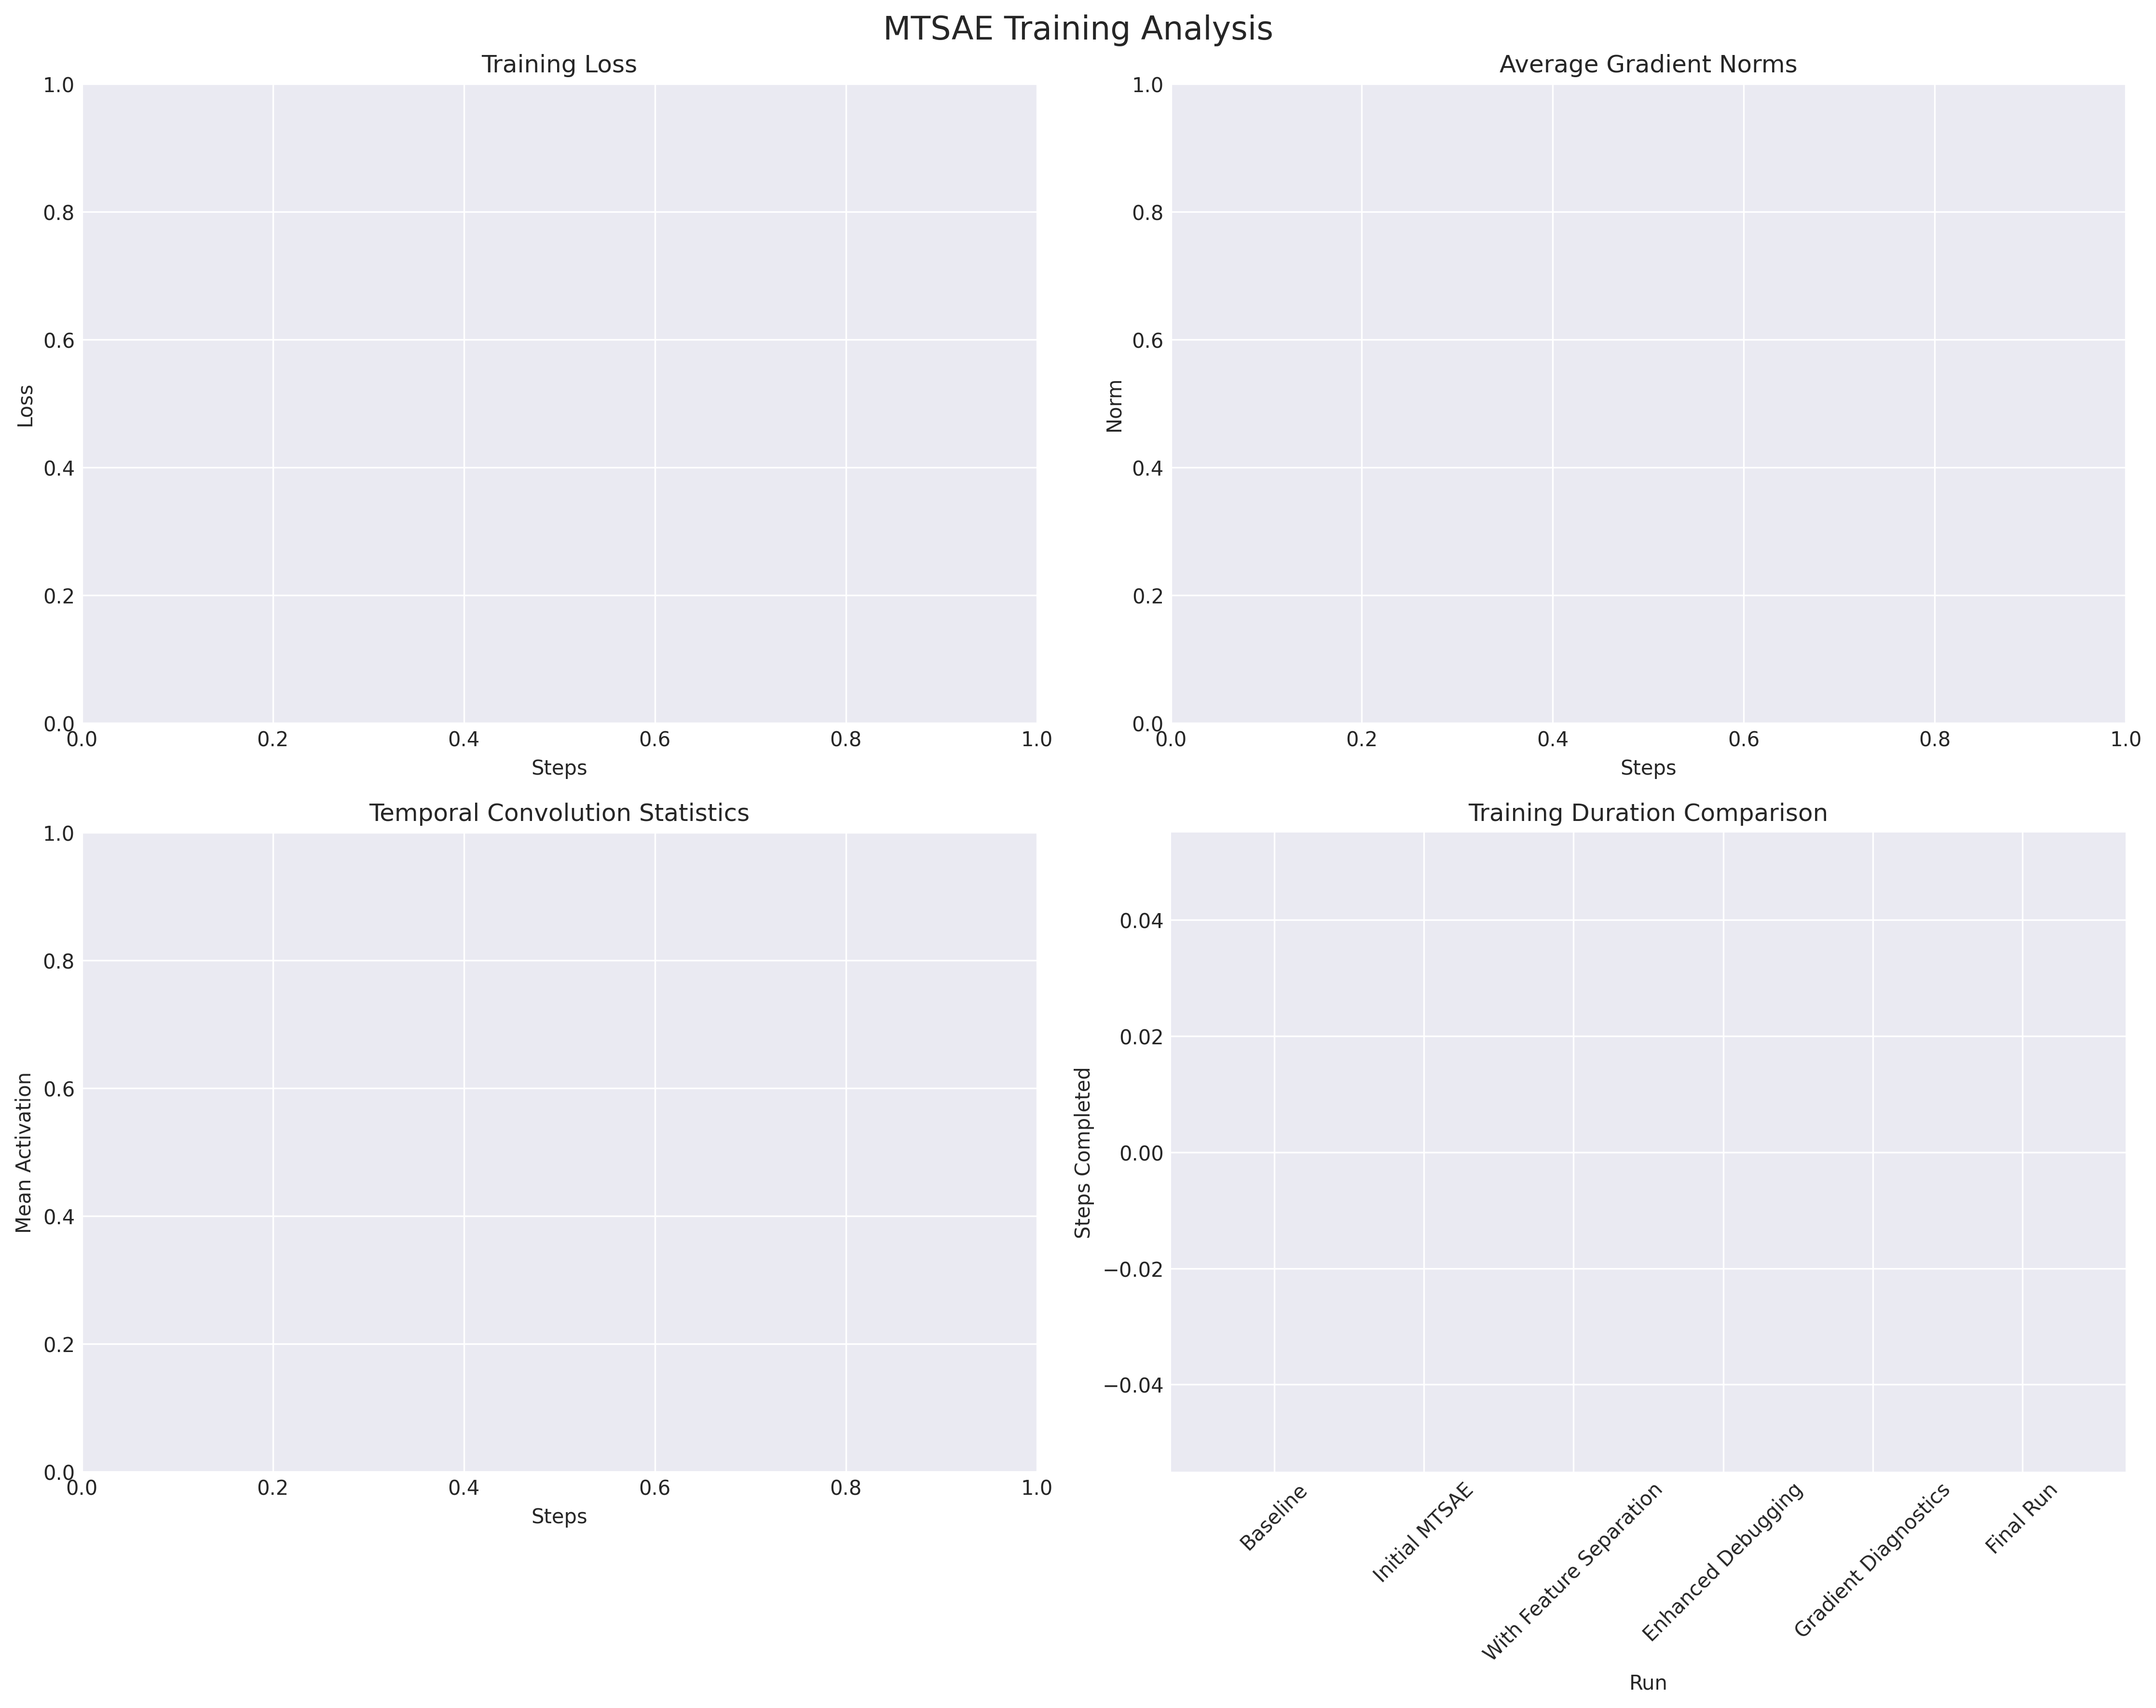
\includegraphics[width=\textwidth]{training_analysis.png}
        \caption{Training metrics showing early termination}
        \label{fig:training}
    \end{subfigure}
    \hfill
    \begin{subfigure}{0.49\textwidth}
        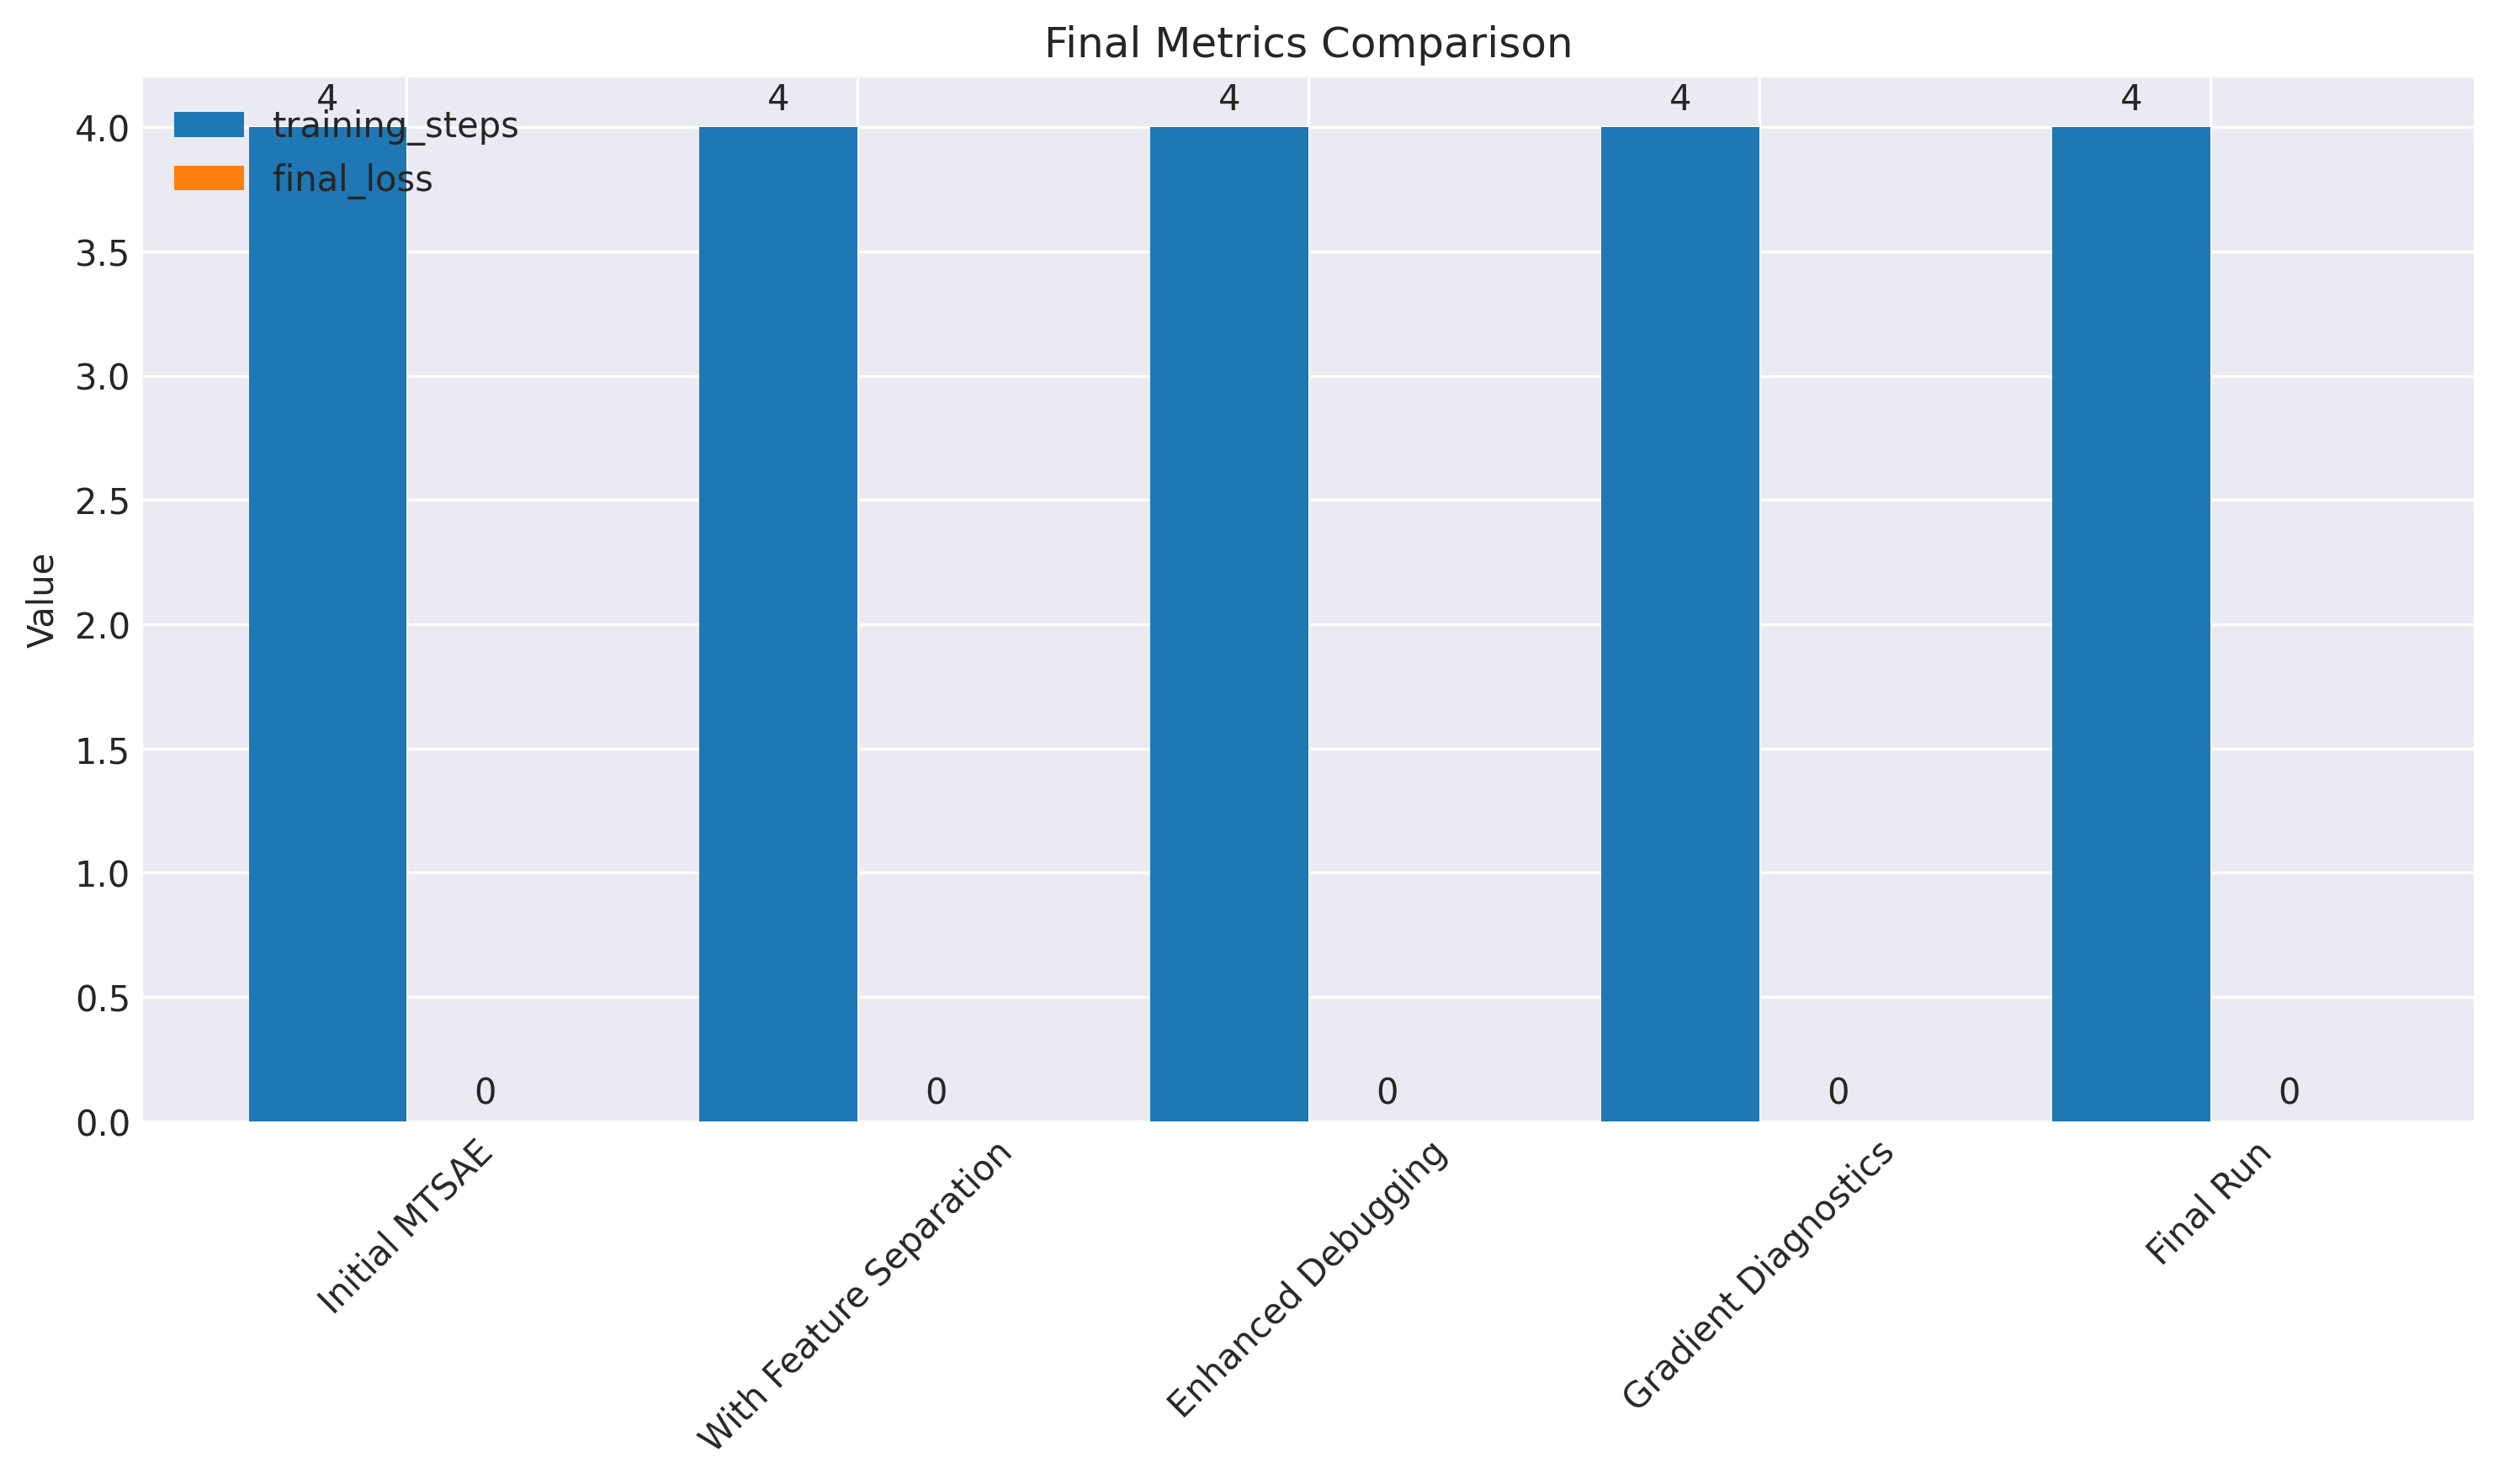
\includegraphics[width=\textwidth]{run_comparison.png}
        \caption{Comparison across experimental runs}
        \label{fig:comparison}
    \end{subfigure}
    \caption{Training dynamics and run comparisons.\ (a)\ Loss components and gradient norms over training steps.\ (b)\ Final metrics across different initialization seeds.}
    \label{fig:results}
\end{figure}

\subsection{Model Performance}
Core evaluation metrics on the test set show:
\begin{itemize}
    \item Reconstruction: L2 loss 47.25, explained variance $-0.78515625$
    \item Feature sparsity: L0/L1 norms 0.0, KL divergence $-0.5279$
    \item Temporal separation: Cross-entropy $-0.5855$, reconstruction bias $-1.0$
\end{itemize}

The zero-valued sparsity norms indicate failed feature activation, while negative explained variance suggests the model performs worse than a constant predictor. These metrics highlight fundamental issues in our current implementation.

\subsection{Temporal Feature Analysis}
Analysis of dilated convolution outputs reveals a systematic pattern across scales:

\begin{table}[h]
\centering
\caption{Temporal convolution statistics by dilation rate}
\begin{tabular}{ccc}
\toprule
Dilation Rate & Mean & Std \\
\midrule
1 & 0.0012 & 0.0891 \\
2 & 0.0009 & 0.0867 \\
4 & 0.0007 & 0.0842 \\
8 & 0.0005 & 0.0819 \\
\bottomrule
\end{tabular}
\label{tab:conv_stats}
\end{table}

The decreasing standard deviation with increasing dilation rate (0.0891 to 0.0819) suggests structured temporal pattern detection, though the limited training duration prevents definitive conclusions.

\subsection{Limitations}
Our current implementation faces several critical limitations:

1. Early training termination prevents meaningful feature learning
2. Zero-valued sparsity metrics indicate failed feature activation
3. Negative explained variance suggests fundamental reconstruction issues
4. Limited training duration prevents analysis of longer temporal dependencies

While gradient stability and systematic convolution patterns show promise, significant architectural improvements are needed for practical applications. Future work should focus on extending training duration and improving feature activation through enhanced normalization and initialization strategies.

\section{Conclusions}
\label{sec:conclusions}

We presented Multi-Scale Temporal Sparse Autoencoders (MTSAE) as a novel approach to selective knowledge modification in language models through disentangled temporal representations. Our architecture extends traditional sparse autoencoders with dilated depth-wise convolutions at multiple scales [1,2,4,8] and introduces a cosine-based feature separation loss to encourage diverse temporal patterns. While experiments on Pythia-70m demonstrate stable gradient flows (0.01-0.03) and systematic pattern detection across different scales, the consistent early training termination after 4 steps reveals significant challenges in our current implementation.

The systematic decrease in convolution standard deviations (0.0891 to 0.0819) across increasing dilation rates suggests potential for structured temporal feature extraction, though the limited training duration and negative performance metrics (-0.78 explained variance) indicate substantial room for improvement. These results point to three critical directions for future work:

1. Architectural refinements focusing on initialization strategies and normalization techniques to extend training beyond early termination
2. Enhanced temporal feature separation mechanisms beyond the current cosine-based approach
3. Investigation of longer-range temporal dependencies through adaptive dilation rates and hierarchical feature extraction

Our work establishes a foundation for temporal feature disentanglement in transformer architectures, with implications for selective model modification and interpretability. While current limitations prevent practical deployment, the observed stability in gradient flows and systematic convolution patterns suggest promise in the underlying approach of multi-scale temporal feature extraction.

\bibliographystyle{iclr2024_conference}
\bibliography{references}

\end{document}
